\chapter{Markov Decision Process}

\section{Markov Processes}


Markov Decision Processes (MDPs) provide the formal mathematical framework for describing environments in reinforcement learning. This formalism captures the essential structure of sequential decision-making problems where an agent interacts with an environment over discrete time steps.

The fundamental assumption underlying MDPs is that the environment is fully observable, meaning the agent has complete access to all information necessary to understand the current state of the system. This complete observability ensures that the current state contains all relevant information needed to make optimal decisions and predict future outcomes.

The current state completely characterizes the process, embodying all the information from the history that is relevant for future decision-making. This property eliminates the need to maintain extensive historical records, as the present state provides sufficient information for optimal action selection.

The versatility of the MDP framework becomes apparent when considering that almost all reinforcement learning problems can be formalized as MDPs. Even scenarios that initially appear to violate MDP assumptions can often be transformed into the MDP framework. Partially observable problems can be converted into MDPs by expanding the state space to include belief states or by using recurrent neural networks to maintain internal memory. Bandit problems represent a special case of MDPs where only a single state exists, demonstrating the framework's broad applicability across different problem complexities.


\subsection{The Markov Property}


The central conceptual foundation of Markov Decision Processes rests on the Markov property, which embodies the principle that "the future is independent of the past, given the present." This fundamental assumption creates a mathematical structure that enables tractable solutions to complex sequential decision problems.

Formally, the Markov property is expressed as:
\begin{equation}
P[S_{t+1}|S_t] = P[S_{t+1}|S_1, \ldots, S_t]
\end{equation}

This equation captures the essence of the memoryless property: what happens next depends only on the current state, not on the sequence of events that led to the current situation. The entire history becomes irrelevant once the current state is known, as all relevant information is encapsulated within the present state.

The state $S_t$ represents a random variable that characterizes the agent's current position or situation within the environment. This state variable captures all the essential features of the environment that influence future transitions and rewards.

Critically, the state $S_t$ serves as a sufficient statistic of the future. This means that the current state contains all the information needed to predict future developments, making it unnecessary to consider the path taken to reach this state. This property dramatically simplifies both the mathematical analysis and computational implementation of learning algorithms, as it reduces the potentially infinite complexity of history-dependent decision making to a manageable state-based framework.


\subsection{State Transition Matrix}


The mathematical structure of Markov processes can be applied to any problem that satisfies the Markov property. The dynamics of state transitions are captured through transition probabilities that define how the system evolves over time.

For a Markov state $s$ and successor state $s'$, the state transition probability is defined by:
\begin{equation}
\mathcal{P}_{ss'} = \mathbb{P}[S_{t+1} = s' | S_t = s]
\end{equation}

This probability quantifies the likelihood of transitioning from state $s$ to state $s'$ in a single time step, providing a complete specification of the system's stochastic dynamics.

Given a current state $s$, the state transition matrix defines the probability distribution over all possible next states $s'$. This matrix representation provides a comprehensive characterization of the environment's dynamics and defines the complete structure of the Markov problem.

The state transition matrix $\mathcal{P}$ takes the form:
\begin{equation}
\mathcal{P} = \begin{pmatrix}
\mathcal{P}_{11} & \cdots & \mathcal{P}_{1n} \\
\vdots & \ddots & \vdots \\
\mathcal{P}_{n1} & \cdots & \mathcal{P}_{nn}
\end{pmatrix}
\end{equation}

Each row of this matrix corresponds to a current state, while each column represents a possible next state. The entry $\mathcal{P}_{ij}$ specifies the probability of transitioning from state $i$ to state $j$. Since these represent probability distributions, each row sums to one, ensuring that the system must transition to some next state with certainty.

This matrix representation enables efficient computation of multi-step transition probabilities through matrix multiplication, facilitates analysis of long-term system behavior, and provides the foundation for value iteration and policy evaluation algorithms in reinforcement learning.


\subsection{Markov Process}


A Markov process represents a memoryless random process, consisting of a sequence of random states $S_1, S_2, \ldots$ that satisfy the Markov property. This mathematical construct provides the foundation for understanding stochastic systems where future evolution depends only on the current state.

Formally, a Markov process is defined as a tuple $\langle \mathcal{S}, \mathcal{P} \rangle$, where:
\begin{compactitemize}
\item $\mathcal{S}$ is a finite set of states representing all possible configurations of the system
\item $\mathcal{P}$ is a state transition probability matrix where $\mathcal{P}_{ss'} = \mathbb{P}[S_{t+1} = s' | S_t = s]$
\end{compactitemize}

At this level of abstraction, the process includes no actions, meaning there is no decision-maker influencing the system's evolution. The system transitions between states according to the fixed probabilities specified in the transition matrix, without any external control or intervention.

Similarly, no rewards are present in a basic Markov process. The system simply evolves through its state space without any notion of desirable or undesirable outcomes. This represents the simplest form of stochastic process that maintains the Markov property.

Despite these limitations, Markov processes provide crucial insights into system dynamics and serve as building blocks for more complex formulations that incorporate decision-making and reward structures. Understanding Markov processes enables the development of intuition about state-based systems and provides the mathematical foundation for Markov Decision Processes.


\subsection{Example: Student Markov Chain}


To illustrate the concepts of Markov processes, consider a student's daily activity patterns modeled as a Markov chain. This example demonstrates how real-world scenarios can be abstracted into mathematical frameworks while maintaining essential behavioral characteristics.

The student's possible states include:
\begin{compactitemize}
\item Class 1, Class 2, Class 3: Different academic activities
\item Pass: Successfully completing coursework
\item Pub: Social activities
\item TikTok: Social media engagement
\item Sleep: Rest periods
\end{compactitemize}

The transition probabilities capture realistic behavioral patterns, and there are show below with the example scheme.



\begin{figure}[H]
    \centering
    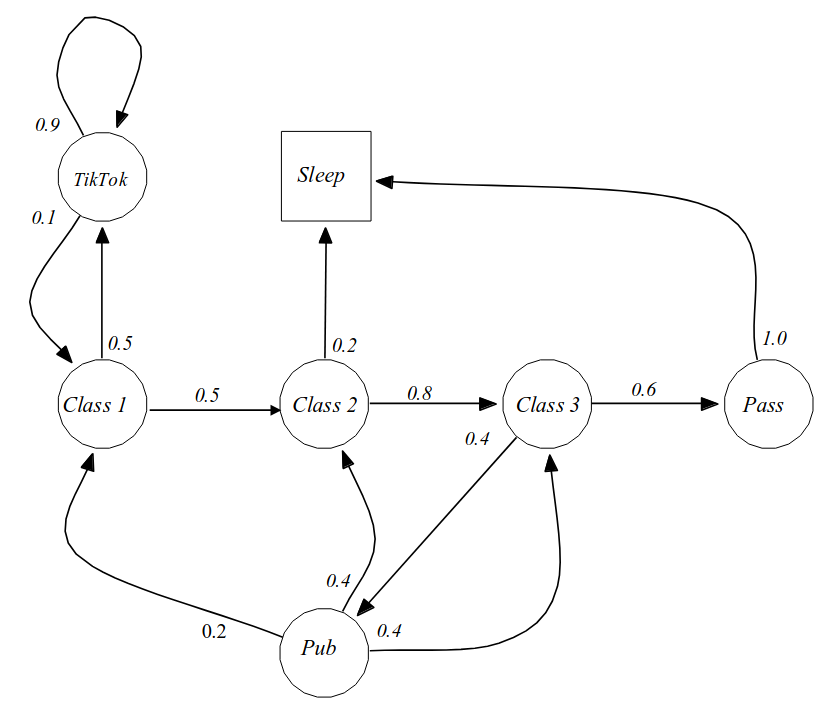
\includegraphics[width=0.6\textwidth]{images/student_chain.png}
    \caption{Student Markov Chain illustrating states and transition probabilities.}
    \label{fig:student_markov_chain}
\end{figure}

\subsubsection{Sample Episodes}

Sampling from this Markov chain generates random sequences of variable length that reflect the stochastic nature of student behavior. Each sample represents a possible trajectory through the state space, determined by the transition probabilities.

Example episodes include:
\begin{compactitemize}
\item C1 → C2 → C3 → Pass → Sleep
\item C1 → TK → TK → C1 → C2 → Sleep  
\item C1 → TK → TK → C1 → C2 → C3 → Pub → C1 → TK → TK → TK → C1 → C2 → C3 → Pub → C2 → Sleep
\end{compactitemize}

These episodes demonstrate several important characteristics of Markov processes. The first episode shows an ideal progression through all class states to successful completion. The second episode illustrates how distractions (TikTok) can interrupt but not necessarily prevent eventual progress. The third episode reveals the complex, potentially lengthy paths that can result from repeated cycles between productive and unproductive states.

The variable length of these episodes reflects the stochastic nature of the process and the presence of absorbing states that terminate the sequence. This variability captures the uncertainty inherent in modeling complex behavioral systems while maintaining the mathematical tractability provided by the Markov property.


\subsubsection{Transition Matrix Representation}

The complete dynamics of the Student Markov Chain can be represented in matrix form, providing a comprehensive specification of all possible state transitions and their associated probabilities.

\begin{equation}
\mathcal{P} = \begin{array}{c|ccccccc}
 & C1 & C2 & C3 & Pass & Pub & TK & Sleep \\
\hline
C1 & 0 & 0.5 & 0 & 0 & 0 & 0.5 & 0 \\
C2 & 0 & 0 & 0.8 & 0 & 0.4 & 0 & 0.2 \\
C3 & 0 & 0 & 0 & 0.6 & 0.4 & 0 & 0 \\
Pass & 0 & 0 & 0 & 0 & 0 & 0 & 1.0 \\
Pub & 0.2 & 0 & 0 & 0 & 0.4 & 0 & 0.4 \\
TK & 0.1 & 0 & 0 & 0 & 0 & 0.9 & 0 \\
Sleep & 0 & 0 & 0 & 0 & 0 & 0 & 1.0
\end{array}
\end{equation}

This matrix representation reveals several important structural properties. Each row represents a current state and sums to 1.0, ensuring that transition probabilities form valid probability distributions. The diagonal elements show self-transition probabilities, with high values for TikTok (0.9) indicating strong tendency to remain distracted, and values of 1.0 for Pass and Sleep indicating absorbing states.

The sparsity of the matrix reflects the realistic constraint that not all state transitions are possible or likely. For example, there are no direct transitions from Sleep to active states, and the Pass state only transitions to Sleep, representing the natural conclusion of academic activities.

This matrix enables computation of long-term behavior through matrix powers, analysis of steady-state distributions, and calculation of expected hitting times between states. Such analyses provide insights into the long-term consequences of different behavioral patterns and the overall structure of the system dynamics.


\section{Markov Reward Process}


A Markov Reward Process (MRP) extends the concept of a Markov Process by associating a reward with each state. This framework introduces the notion of value, allowing us to evaluate the desirability of states in terms of expected future rewards.

Formally, an MRP is defined as a tuple $\langle \mathcal{S}, \mathcal{P}, \mathcal{R}, \gamma \rangle$, where:
\begin{itemize}
    \item $\mathcal{S}$ is a finite set of states
    \item $\mathcal{P}$ is the state transition probability matrix
    \item $\mathcal{R}$ is a reward function, where $\mathcal{R}_s = \mathbb{E}[R_{t+1} | S_t = s]$
    \item $\gamma$ is a discount factor, $\gamma \in [0,1]$, representing the present value of future rewards
\end{itemize}

The total return from a state $S_t$ is defined as the discounted sum of future rewards:
\begin{equation}
G_t = R_{t+1} + \gamma R_{t+2} + \gamma^2 R_{t+3} + \cdots
= \sum_{k=0}^{\infty} \gamma^k R_{t+k+1}
\end{equation}

The \textbf{state-value function} $v(s)$ represents the expected return starting from state $s$:
\begin{equation}
v(s) = \mathbb{E}[G_t \mid S_t = s] 
= \mathbb{E}[R_{t+1} + \gamma v(S_{t+1}) \mid S_t = s]
\end{equation}

\begin{figure}[H]
    \centering
    \begin{minipage}{0.45\textwidth}
        \centering
        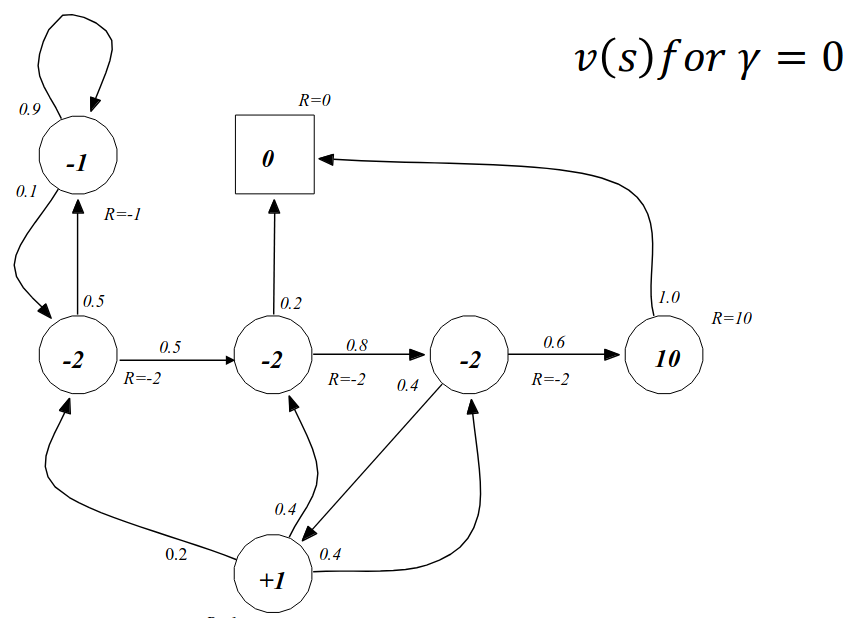
\includegraphics[width=\textwidth]{images/gamm0.png}
        \caption{Student Markov Chain with $\gamma=0$}
        \label{fig:STMCR}
    \end{minipage}
    \hfill
    \begin{minipage}{0.45\textwidth}
        \centering
        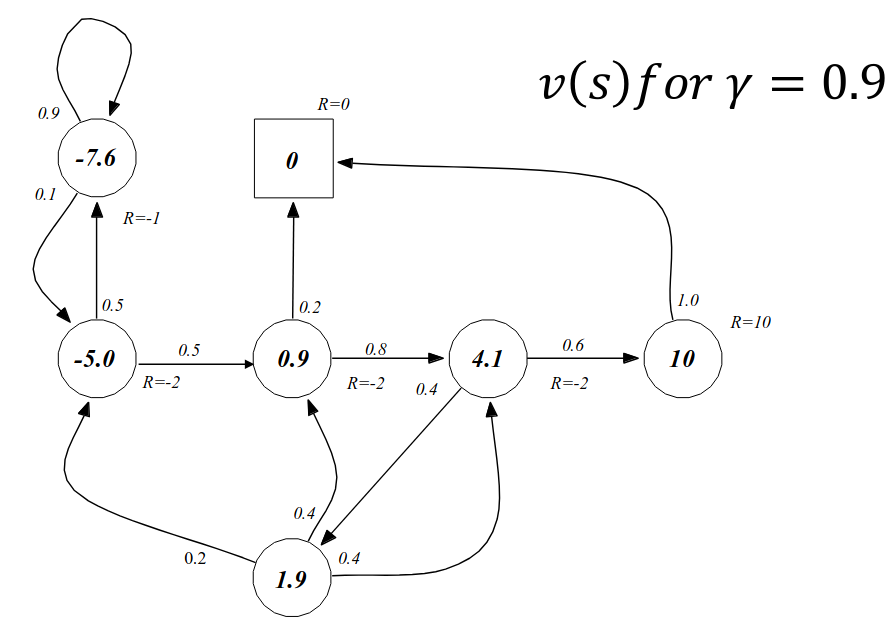
\includegraphics[width=\textwidth]{images/gamma9.png}
        \caption{Student Markov Chain with $\gamma=0.9$}
        \label{fig:STMCR}
    \end{minipage}
    \label{STMCR}
\end{figure}

\subsection{Bellman Equation for MRPs}

The fundamental idea behind the Bellman equation for Markov Reward Processes is that the value function admits a \textbf{recursive decomposition}. The value of a state does not depend directly on the entire future sequence of rewards, but can be expressed as the sum of two contributions: the immediate reward and the expected value of the next state, appropriately discounted.

By definition, the value function of a state $s$ is the expected value of the return starting from that state:
\[
v(s) = \mathbb{E}\!\left[ G_t \mid S_t = s \right]
\]
where the return is defined as:
\[
G_t = R_{t+1} + \gamma R_{t+2} + \gamma^2 R_{t+3} + \dots
\]

Making this definition explicit, we obtain:
\[
v(s)
=
\mathbb{E}
\left[
R_{t+1}
+ \gamma R_{t+2}
+ \gamma^2 R_{t+3}
+ \dots
\;\middle|\;
S_t = s
\right]
\]

Grouping the first term and factoring out $\gamma$, the return can be rewritten as:
\[
v(s)
=
\mathbb{E}
\left[
R_{t+1}
+ \gamma
\left(
R_{t+2}
+ \gamma R_{t+3}
+ \dots
\right)
\;\middle|\;
S_t = s
\right]
\]

Observing that the expression in parentheses coincides with the return starting from time $t+1$, we obtain:
\[
v(s)
=
\mathbb{E}
\left[
R_{t+1}
+ \gamma G_{t+1}
\;\middle|\;
S_t = s
\right]
\]

Since $G_{t+1}$ is, by definition, the return starting from state $S_{t+1}$, the term can be expressed as the value function of the next state:
\[
v(s)
=
\mathbb{E}
\left[
R_{t+1}
+ \gamma v(S_{t+1})
\;\middle|\;
S_t = s
\right]
\]

This equation compactly expresses the principle according to which the overall value of a state is given by the expected immediate reward plus the discounted value of the next state.

In the case of a Markov Reward Process, the expected reward and the transition probabilities depend only on the current state. Denoting by $\mathcal{R}_s$ the average reward associated with state $s$ and by $\mathcal{P}_{ss'}$ the transition probability from $s$ to $s'$, the expectation can be made explicit:
\[
v(s)
=
\mathcal{R}_s
+
\gamma
\sum_{s' \in \mathcal{S}}
\mathcal{P}_{ss'} \, v(s')
\]

This is the \textbf{Bellman equation for Markov Reward Processes}. It provides a recursive characterization of the value function and is the theoretical foundation of all prediction and control algorithms in Reinforcement Learning.

\subsection{Matrix Form}


In matrix notation, the Bellman equation is:
\begin{equation}
v = \mathcal{R} + \gamma \mathcal{P} v \quad \Rightarrow \quad v = (I - \gamma \mathcal{P})^{-1} \mathcal{R}
\end{equation}

For example, consider a small MRP with 3 states:
\[
\mathcal{P} =
\begin{bmatrix}
0.5 & 0.2 & 0.3 \\
0.1 & 0.9 & 0.0 \\
0.4 & 0.4 & 0.2
\end{bmatrix}, \quad
\mathcal{R} =
\begin{bmatrix}
-1 \\
10 \\
0
\end{bmatrix}, \quad \gamma = 1
\]

The value vector $v$ can be computed as:
\[
v =
\begin{bmatrix}
v_1 \\
v_2 \\
v_3
\end{bmatrix} =
\mathcal{R} + \gamma \mathcal{P} v
=
\begin{bmatrix}
-1 \\
10 \\
0
\end{bmatrix} +
\begin{bmatrix}
0.5 & 0.2 & 0.3 \\
0.1 & 0.9 & 0.0 \\
0.4 & 0.4 & 0.2
\end{bmatrix}
\begin{bmatrix}
v_1 \\
v_2 \\
v_3
\end{bmatrix}
\]



This illustrates how the Bellman equation can be written in matrix form, which is particularly useful for computational solutions of MRPs. The computation complexity is $O(n^3)$ due to the matrix inversion, where $n$ is the number of states. Direct solution is possible only for small MRPs.
There are many iterative methods for latge MRPs,such as:
\begin{compactitemize}
    \item Dynamic Programming
    \item Monte-Carlo methods
    \item Temporal-Difference Learning
\end{compactitemize}


\section{Markov Decision Process}


While Markov Reward Processes provide a framework for evaluating states in terms of expected rewards, they lack the crucial element of agency. In MRPs, the agent has no control over the system's evolution and simply flows through the environment according to the fixed transition probabilities specified in $\mathcal{P}$. This limitation necessitates the introduction of decision-making capabilities.

A Markov Decision Process (MDP) extends the MRP framework by incorporating actions and decision-making, creating an environment where an agent can influence the system's evolution through deliberate choices. MDPs represent the mathematical foundation for sequential decision-making under uncertainty, where all states maintain the Markov property.

Formally, an MDP is defined as a tuple $\langle \mathcal{S}, \mathcal{A}, \mathcal{P}, \mathcal{R}, \gamma \rangle$, where:
\begin{compactitemize}
\item $\mathcal{S}$ is a finite set of states representing all possible configurations of the environment
\item $\mathcal{A}$ is a finite set of actions available to the agent
\item $\mathcal{P}$ is a state transition probability matrix, where $\mathcal{P}_{ss'}^a = \mathbb{P}[S_{t+1} = s' | S_t = s, A_t = a]$
\item $\mathcal{R}$ is a reward function, where $\mathcal{R}_s^a = \mathbb{E}[R_{t+1} | S_t = s, A_t = a]$
\item $\gamma$ is a discount factor, $\gamma \in [0,1]$
\end{compactitemize}

The critical distinction from MRPs lies in the action-dependent nature of both transitions and rewards. The probability of transitioning to state $s'$ now depends not only on the current state $s$ but also on the action $a$ chosen by the agent. Similarly, the expected reward depends on both the current state and the selected action, providing the agent with the ability to influence both immediate rewards and future state evolution.



\begin{figure}[H]
    \centering
    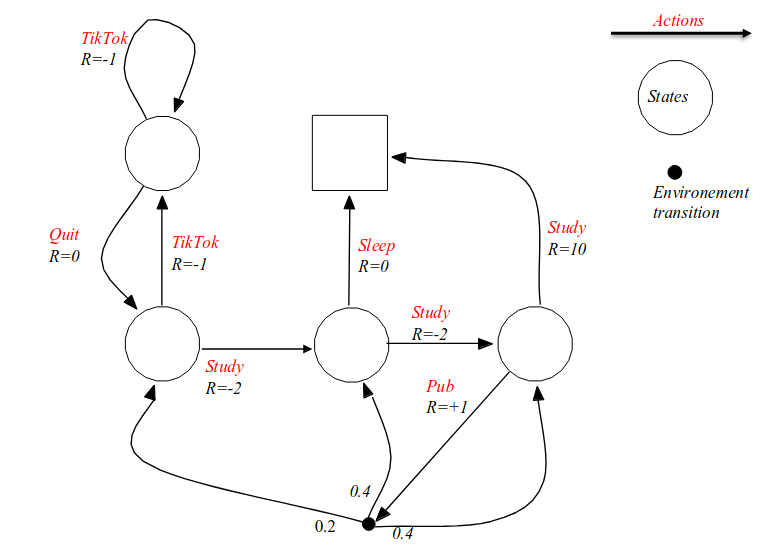
\includegraphics[width=0.6\textwidth]{images/MDP_chain.png}
    \caption{Student MDP Chain.}
    \label{fig:student_markov_chain}
\end{figure}


    \textbf{Note:}The black point in the figure above rappresent an enviroment transition, this is not under the control of the agent. So with a some probability the agent will move to one of the possible next states.


\subsection{Policy}


The concept of agency in MDPs is formalized through the notion of a policy, which defines how an agent behaves in the environment. A policy serves as the decision-making mechanism that maps states to actions, providing a complete specification of the agent's behavior strategy.

A policy $\pi$ is formally defined as a distribution over actions given states:
\begin{equation}
\pi(a|s) = \mathbb{P}[A_t = a | S_t = s]
\end{equation}

This probabilistic formulation allows for both deterministic policies, where a single action is chosen with probability 1, and stochastic policies, where actions are selected according to a probability distribution. The policy completely defines the agent's behavior, as it specifies how the agent chooses actions based solely on the current state.

Several important properties characterize MDP policies. First, policies depend only on the current state, not on the history of states, actions, or rewards. This memoryless property aligns with the Markov assumption and ensures that optimal decision-making requires only knowledge of the present situation.

Second, policies focus exclusively on future rewards, disregarding past experiences in the decision-making process. This forward-looking perspective reflects the goal-oriented nature of reinforcement learning, where the objective is to maximize expected future returns rather than to optimize past performance.

Finally, policies are stationary, meaning they are time-independent. The same policy applies regardless of when a decision is made, providing consistency across different time steps and enabling the development of stable behavioral strategies.


\subsection{Value Functions}


Value functions provide the mathematical foundation for evaluating the quality of states and actions under a given policy. These functions quantify the expected future performance of different choices, enabling rational decision-making in uncertain environments.

The \textbf{state-value function} $v^\pi(s)$ represents the expected return when starting from state $s$ and subsequently following policy $\pi$:
\begin{equation}
v_\pi(s) = \mathbb{E}_\pi[G_t | S_t = s]
\end{equation}

This function captures the long-term value of being in a particular state under a specific policy, incorporating both immediate rewards and the discounted value of all future states that may be visited.

The \textbf{action-value function} $q^\pi(s,a)$ extends this concept by evaluating the expected return when starting from state $s$, taking action $a$, and then following policy $\pi$:
\begin{equation}
q_\pi(s,a) = \mathbb{E}_\pi[G_t | S_t = s, A_t = a]
\end{equation}

The action-value function provides more granular information by distinguishing between the values of different actions in the same state. This additional detail enables the comparison of alternative actions and supports the development of improved policies through action selection based on expected returns.

These value functions form the basis for policy evaluation, policy improvement, and ultimately the discovery of optimal policies that maximize expected returns across all states and situations.

\subsubsection{Bellman Equations for MDPs}

In Markov Decision Processes too, the value function admits a recursive decomposition, analogous to that of Markov Reward Processes, with the fundamental difference that the dynamics of the environment now also depend on the actions selected according to a policy $\pi$.

Consider a fixed policy $\pi$. The state-value function $v_\pi(s)$ is defined as the expected return starting from state $s$ and following the policy $\pi$:
\[
v_\pi(s) = \mathbb{E}_\pi \big[ G_t \mid S_t = s \big]
\]

Using the definition of return and separating the first term, the value of the state can be expressed as:
\[
v_\pi(s)
=
\mathbb{E}_\pi
\big[
R_{t+1} + \gamma G_{t+1}
\mid S_t = s
\big]
\]

Since $G_{t+1}$ represents the return starting from the next state $S_{t+1}$, we obtain the first form of the Bellman expectation equation:
\[
v_\pi(s)
=
\mathbb{E}_\pi
\big[
R_{t+1} + \gamma v_\pi(S_{t+1})
\mid S_t = s
\big]
\]

In a completely analogous way, it is possible to obtain a recursive decomposition for the action-value function. The function $q_\pi(s,a)$ represents the expected return starting from state $s$, executing action $a$ and then following the policy $\pi$:
\[
q_\pi(s,a)
=
\mathbb{E}_\pi
\big[
R_{t+1} + \gamma q_\pi(S_{t+1}, A_{t+1})
\mid S_t = s, A_t = a
\big]
\]

These relations express the general principle according to which the expected value is given by the immediate reward plus the expected value of the next step.

To make the equations completely explicit, the expectation operator can be eliminated by introducing the policy $\pi$, the reward function $\mathcal{R}$ and the transition probabilities $\mathcal{P}$. The state-value function can be rewritten as a weighted average of the action-value functions:
\[
v_\pi(s) = \sum_{a \in \mathcal{A}} \pi(a \mid s)\, q_\pi(s,a)
\]

In turn, the action-value function satisfies:
\[
q_\pi(s,a)
=
\mathcal{R}_s^a
+
\gamma
\sum_{s' \in \mathcal{S}}
\mathcal{P}_{ss'}^a \, v_\pi(s')
\]

Substituting this expression into the definition of $v_\pi(s)$, we obtain the Bellman expectation equation for the state-value function:
\[
v_\pi(s)
=
\sum_{a \in \mathcal{A}}
\pi(a \mid s)
\left[
\mathcal{R}_s^a
+
\gamma
\sum_{s' \in \mathcal{S}}
\mathcal{P}_{ss'}^a
\, v_\pi(s')
\right]
\]

Analogously, substituting the definition of $v_\pi(s')$ in terms of $q_\pi$, we obtain the Bellman expectation equation for the action-value function:
\[
q_\pi(s,a)
=
\mathcal{R}_s^a
+
\gamma
\sum_{s' \in \mathcal{S}}
\mathcal{P}_{ss'}^a
\sum_{a' \in \mathcal{A}}
\pi(a' \mid s')\, q_\pi(s',a')
\]

These equations completely characterize the evaluation of a policy in an MDP and are the theoretical basis of all policy evaluation algorithms, both model-based and model-free. In particular, they show how the effect of future actions is incorporated into the value through the expectation with respect to the policy $\pi$.

\subsection{Optimal Value Functions}

In a Markov Decision Process, the goal of the control problem is to determine the best performance achievable by the agent over all states. This information is captured by the \textbf{optimal value functions}.

The \textbf{optimal state-value function} is defined as the maximum value achievable starting from state $s$ over all possible policies:
\[
v^*(s) = \max_{\pi} v_\pi(s)
\]

Analogously, the \textbf{optimal action-value function} is defined as the maximum value achievable starting from the state–action pair $(s,a)$ over all policies:
\[
q^*(s,a) = \max_{\pi} q_\pi(s,a)
\]

The optimal value function therefore represents the upper bound of the performance achievable in an MDP. An MDP is said to be \emph{solved} when the optimal value function is known, since an optimal policy can be derived directly from it.
\begin{figure}[H]
    \centering
    \begin{minipage}{0.45\textwidth}
        \centering
        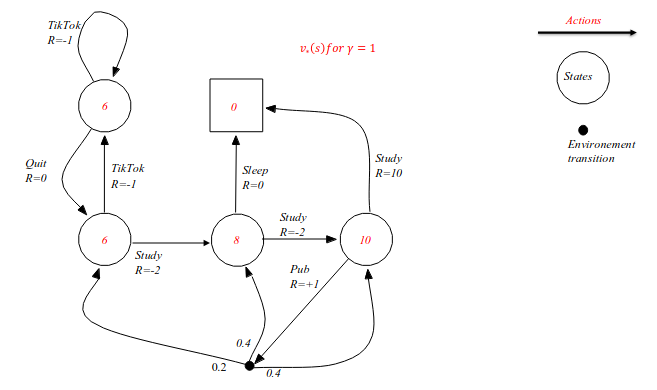
\includegraphics[width=\textwidth]{images/L11.png}
        \caption{Optimal value function for student MDP}
        \label{fig:STMCR}
    \end{minipage}
    \hfill
    \begin{minipage}{0.45\textwidth}
        \centering
        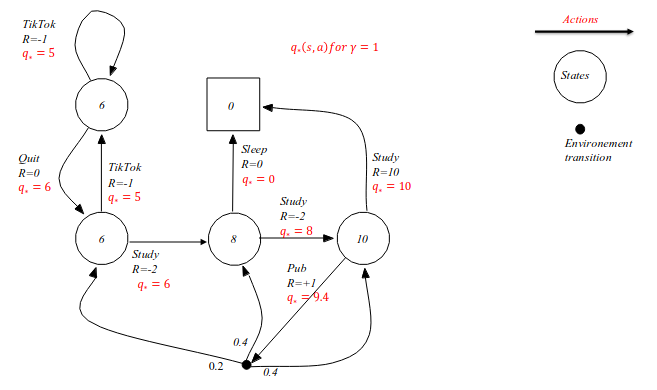
\includegraphics[width=\textwidth]{images/L12.png}
        \caption{Optimal action-value function for Studenr MDP}
        \label{fig:STMCR}
    \end{minipage}
    \label{STMCR}
\end{figure}


\subsection{Optimal Policies}

It is possible to introduce a partial ordering between policies by comparing their respective state values. Given two policies $\pi$ and $\pi'$, we say that:
\[
\pi \ge \pi'
\quad \text{if and only if} \quad
v_\pi(s) \ge v_{\pi'}(s) \quad \forall s \in \mathcal{S}
\]

A fundamental result of Reinforcement Learning states that, for every MDP, \textbf{there exists at least one optimal policy} $\pi^*$ such that:
\[
\pi^* \ge \pi \qquad \forall \pi
\]

All optimal policies share the same optimal value functions:
\[
v_{\pi^*}(s) = v^*(s),
\qquad
q_{\pi^*}(s,a) = q^*(s,a)
\]

A particularly important fact is that, for every MDP, \textbf{there always exists a deterministic optimal policy}. This means that it is not necessary to resort to randomization to obtain optimal behaviour.

If the optimal action-value function is known, an optimal policy can be obtained directly by choosing, in every state, the action that maximizes $q^*(s,a)$:
\[
\pi^*(a \mid s) =
\begin{cases}
1 & \text{if } a \in \arg\max_{a' \in \mathcal{A}} q^*(s,a') \\
0 & \text{otherwise}
\end{cases}
\]

This relation shows that knowing $q^*$ is sufficient to completely determine an optimal policy.


\subsection{Bellman Optimality Equations}

The optimal value functions satisfy a recursive relation called the \textbf{Bellman optimality equation}. Unlike the Bellman expectation equations, in this case the expectation with respect to the policy is replaced by a maximum operation, since the agent is assumed to act optimally.

The Bellman optimality equation for the state-value function is:
\[
v^*(s) = \max_{a \in \mathcal{A}} q^*(s,a)
\]

Explicitly expressing the dynamics of the MDP, the same equation can be written as:
\[
v^*(s)
=
\max_{a \in \mathcal{A}}
\left[
\mathcal{R}_s^a
+
\gamma
\sum_{s' \in \mathcal{S}}
\mathcal{P}_{ss'}^a \, v^*(s')
\right]
\]

Analogously, the Bellman optimality equation for the action-value function is:
\[
q^*(s,a)
=
\mathcal{R}_s^a
+
\gamma
\sum_{s' \in \mathcal{S}}
\mathcal{P}_{ss'}^a
\max_{a' \in \mathcal{A}} q^*(s',a')
\]

These equations completely characterize the control problem in Markov Decision Processes. The functions $v^*$ and $q^*$ are the fixed points of these Bellman operators and are the theoretical foundation of all control algorithms, both model-based and model-free, such as Value Iteration, Policy Iteration, SARSA and Q-learning.
